% Standard Article Definition
\documentclass[]{article}

% Page Formatting
\usepackage[margin=1in]{geometry}
\setlength\parindent{0pt}

% Graphics
\usepackage{graphicx}

% Math Packages
\usepackage{physics}
\usepackage{amsmath, amsfonts, amssymb, amsthm}
\usepackage{mathtools}

% Extra Packages
\usepackage{pdfpages}
\usepackage{hyperref}
% \usepackage{listings}

% Section Heading Settings
% \usepackage{enumitem}
% \renewcommand{\theenumi}{\alph{enumi}}
\renewcommand*{\thesection}{Problem \arabic{section}}
\renewcommand*{\thesubsection}{\arabic{section}\alph{subsection})}
\renewcommand*{\thesubsubsection}{}%\quad \quad \roman{subsubsection})}

\newcommand{\Problem}{\subsubsection*{\textbf{PROBLEM:}}}
\newcommand{\Solution}{\subsubsection*{\textbf{SOLUTION:}}}
\newcommand{\Preliminaries}{\subsubsection*{\textbf{PRELIMINARIES:}}}

%Custom Commands
\newcommand{\N}{\mathbb{N}}
\newcommand{\Z}{\mathbb{Z}}
% \newcommand{\Q}{\mathbb{Q}}
\newcommand{\R}{\mathbb{R}}
\newcommand{\C}{\mathbb{C}}

% \newcommand{\SigAlg}{\mathcal{S}}

% \newcommand{\Rel}{\mathcal{R}}

% \newcommand{\toI}{\xrightarrow{\textsf{\tiny I}}}
% \newcommand{\toS}{\xrightarrow{\textsf{\tiny S}}}
% \newcommand{\toB}{\xrightarrow{\textsf{\tiny B}}}

% \newcommand{\divisible}{ \ \vdots \ }
\newcommand{\st}{\ : \ }

% Theorem Definition
\newtheorem{definition}{Definition}
\newtheorem{assumption}{Assumption}
\newtheorem{theorem}{Theorem}
\newtheorem{lemma}{Lemma}
\newtheorem{proposition}{Proposition}
\newtheorem{remark}{Remark}
% \newtheorem{example}{Example}
% \newtheorem{counterExample}{Counter Example}


%opening
\title{
    MECH 6v29 - Model Predictive Control\\ 
    Homework 1
}
\author{Jonas Wagner\\ jonas.wagner@utdallas.edu}
\date{2023, September 29\textsuperscript{th}}

\begin{document}

\maketitle

\tableofcontents

% Problem 1
\newpage
\section{}

% 1a)
\subsection{}

\begin{figure}[h]
    \centering
    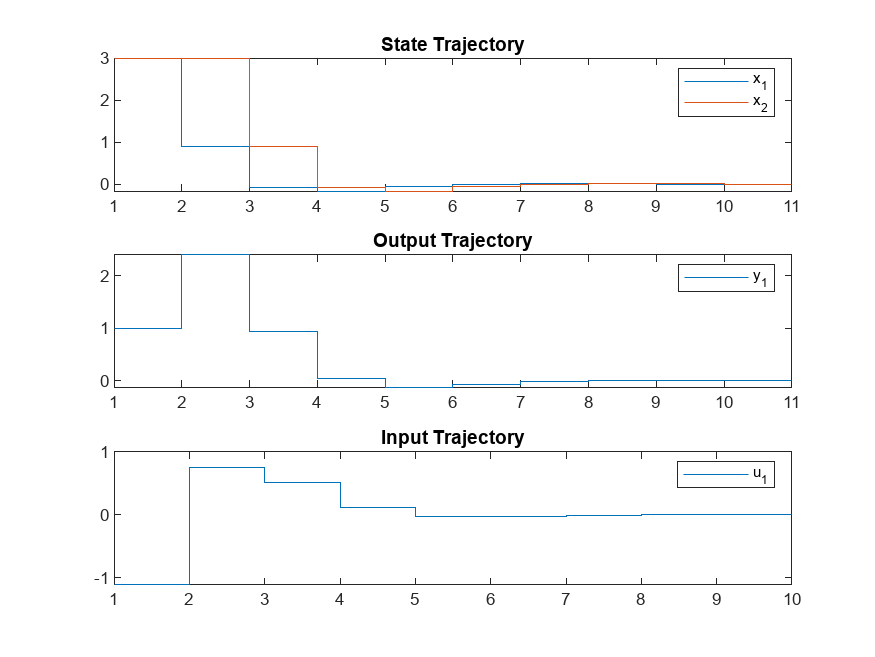
\includegraphics[width = 0.5\textwidth]{figs/pblm1a.png}
    \caption{Problem 1a results}
\end{figure}

The transient behavior is pretty reasonable and has a mild overshoot.
The maximum output is around 2.5 (2.409) and it appears to initially reach the origin after 4 timesteps but takes around 7 to settle.

% 1b)
\subsection{}
\begin{figure}[h]
    \centering
    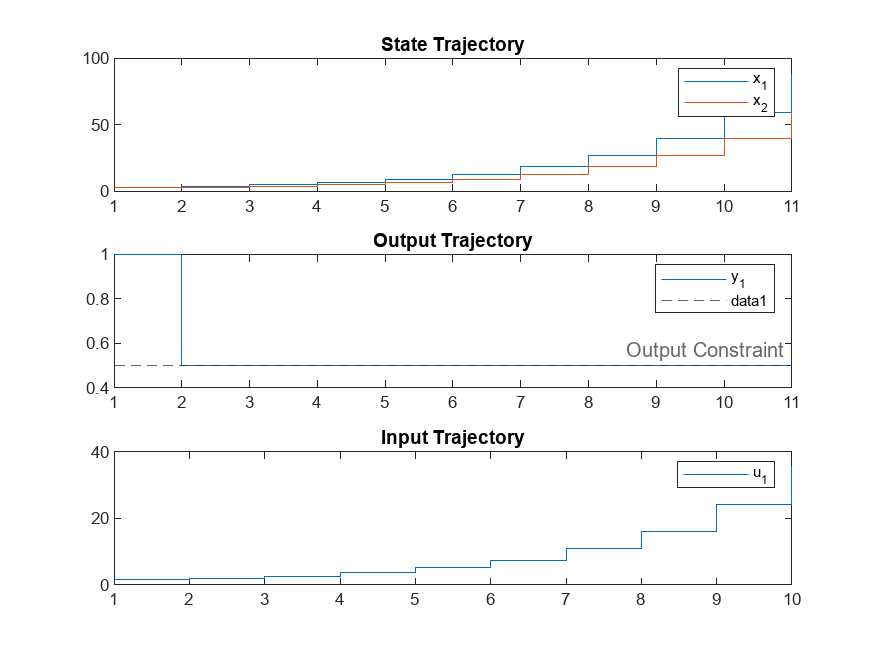
\includegraphics[width = 0.5\textwidth]{figs/pblm1b.png}
    \caption{Problem 1b results}
\end{figure}

The controller is unable to stabilize the system.

Is it possible to tune the cost function matrices? Potentially, although I'm not sure how to explicitly prove this for every case. (Although for this exact initial condition and other parameters I believe taking R = 0 may work)






% See MATLAB results

% The results are not the same, at least for the short prediction horizon

% % 1c)
% \subsection{}
% Se MATLAB Results

% % 1d)
% \subsection{}
% See MATLAB Results

% % 1e)
% \subsection{}
% See MATLAB Results

% From the results, it is clear that the closed-loop system results become more stable as the prediction horizon increases and converges upon the LQR-solution.
% It appears as though the system enters stability around when $N=6$, although I am uncertain if this is always the case, or just for this state specifically.

% This is around half the settling time, so perhaps this would be a good guess.

% % MATLAB
% 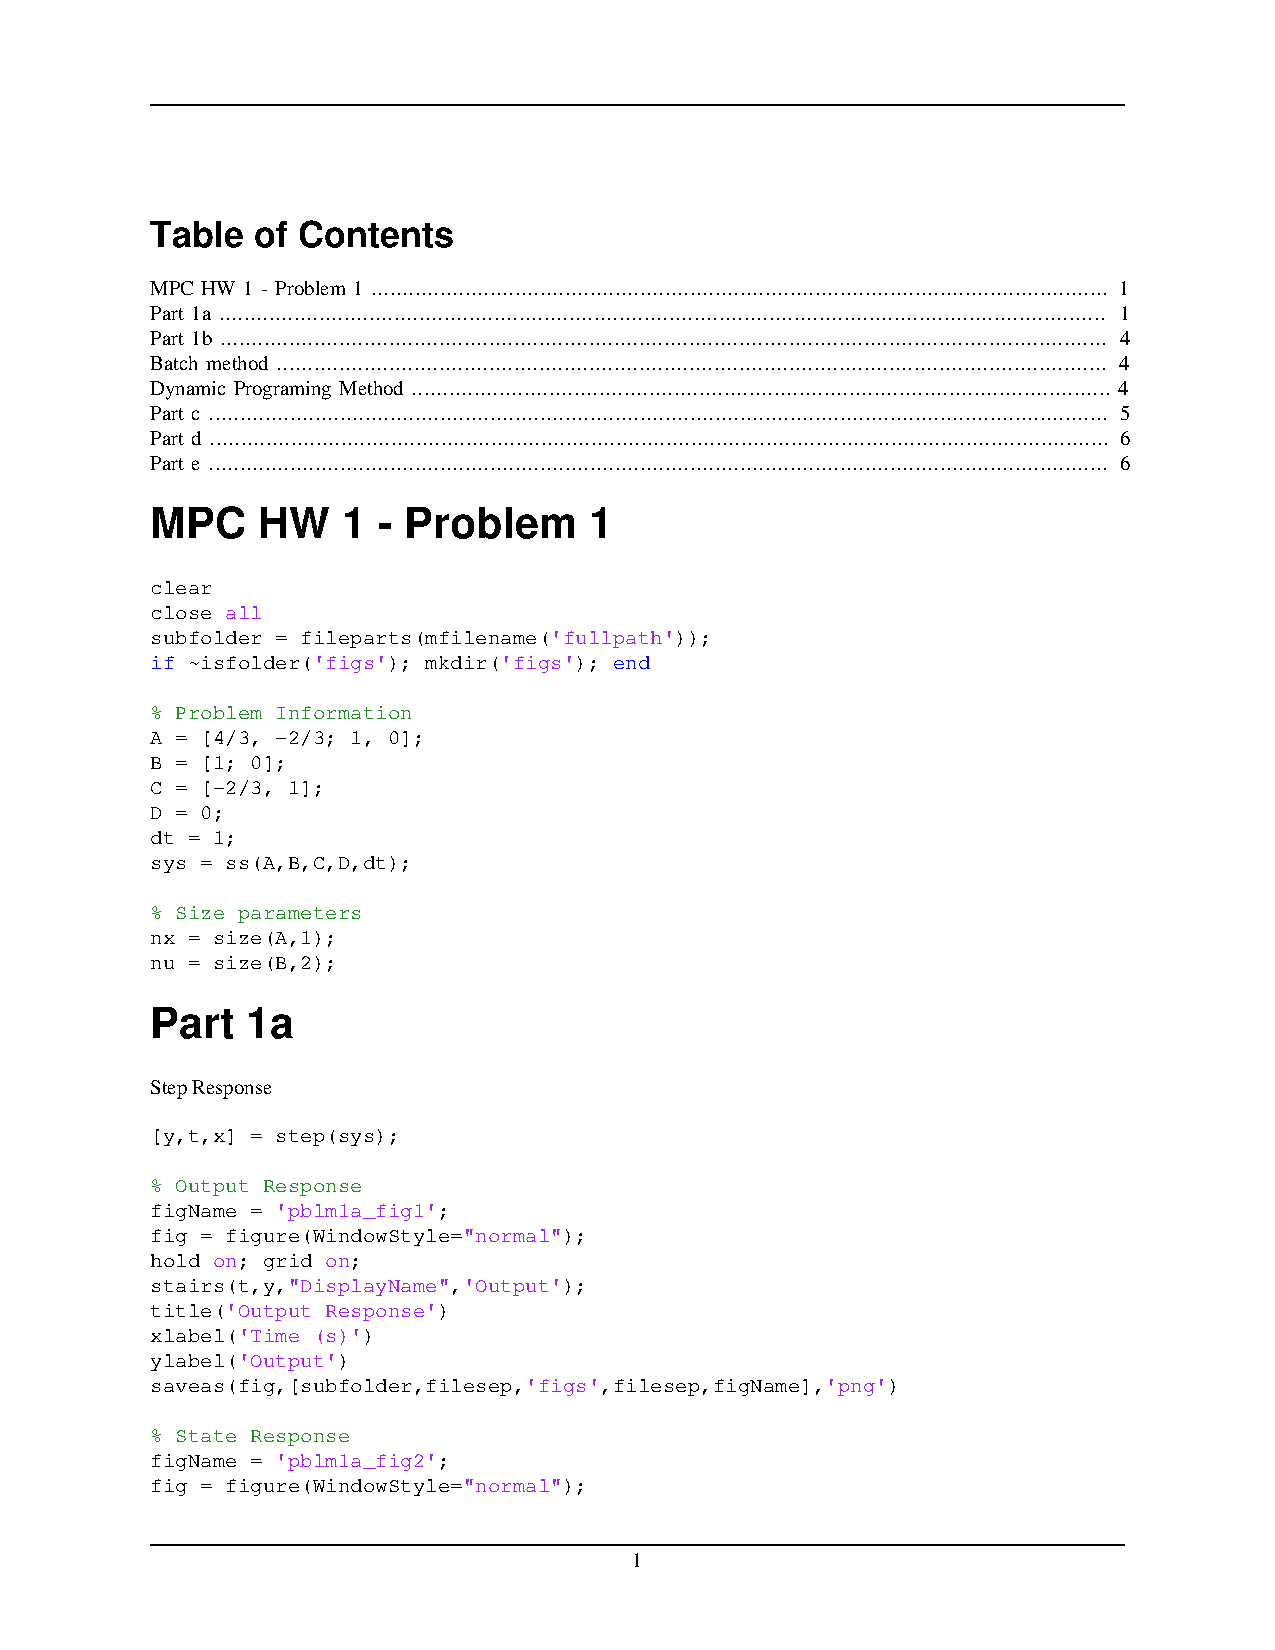
\includepdf[pages=-]{HW1_pblm1.pdf}


% % \textbf{Problem 2:}
% \section{}

% Generally my results to this problem were not as I expected, but I'm pretty sure they are correct given the system listed in the assignment.

% % 2a)
% \subsection{}
% See MATLAB code

% The lack of any major transient behavior is weird, but I'm guessing that this is becouse the lack of constraints allow it to reach it's "steady-state" after only one time-step

% % 2b)
% \subsection{}
% See MATLAB code

% This is a much much better result (as is often expected with increased time-horizons)


% % 2c)
% \subsection{}
% See MATLAB code

% This made it unstable.
% There is no longer enough input constraints to counteract the main response of the system.

% % 2d)
% \subsection{}
% See MATLAB code

% It was unclear whether the input constraints were also to be included, thus both versions were tested.

% When only the state is restricted, the response of the system is just slowed and the input decreases as expected until it reaches zero.
% However, the MPC problem becomes unfeasible when both the input and state constraints are implimented.



% 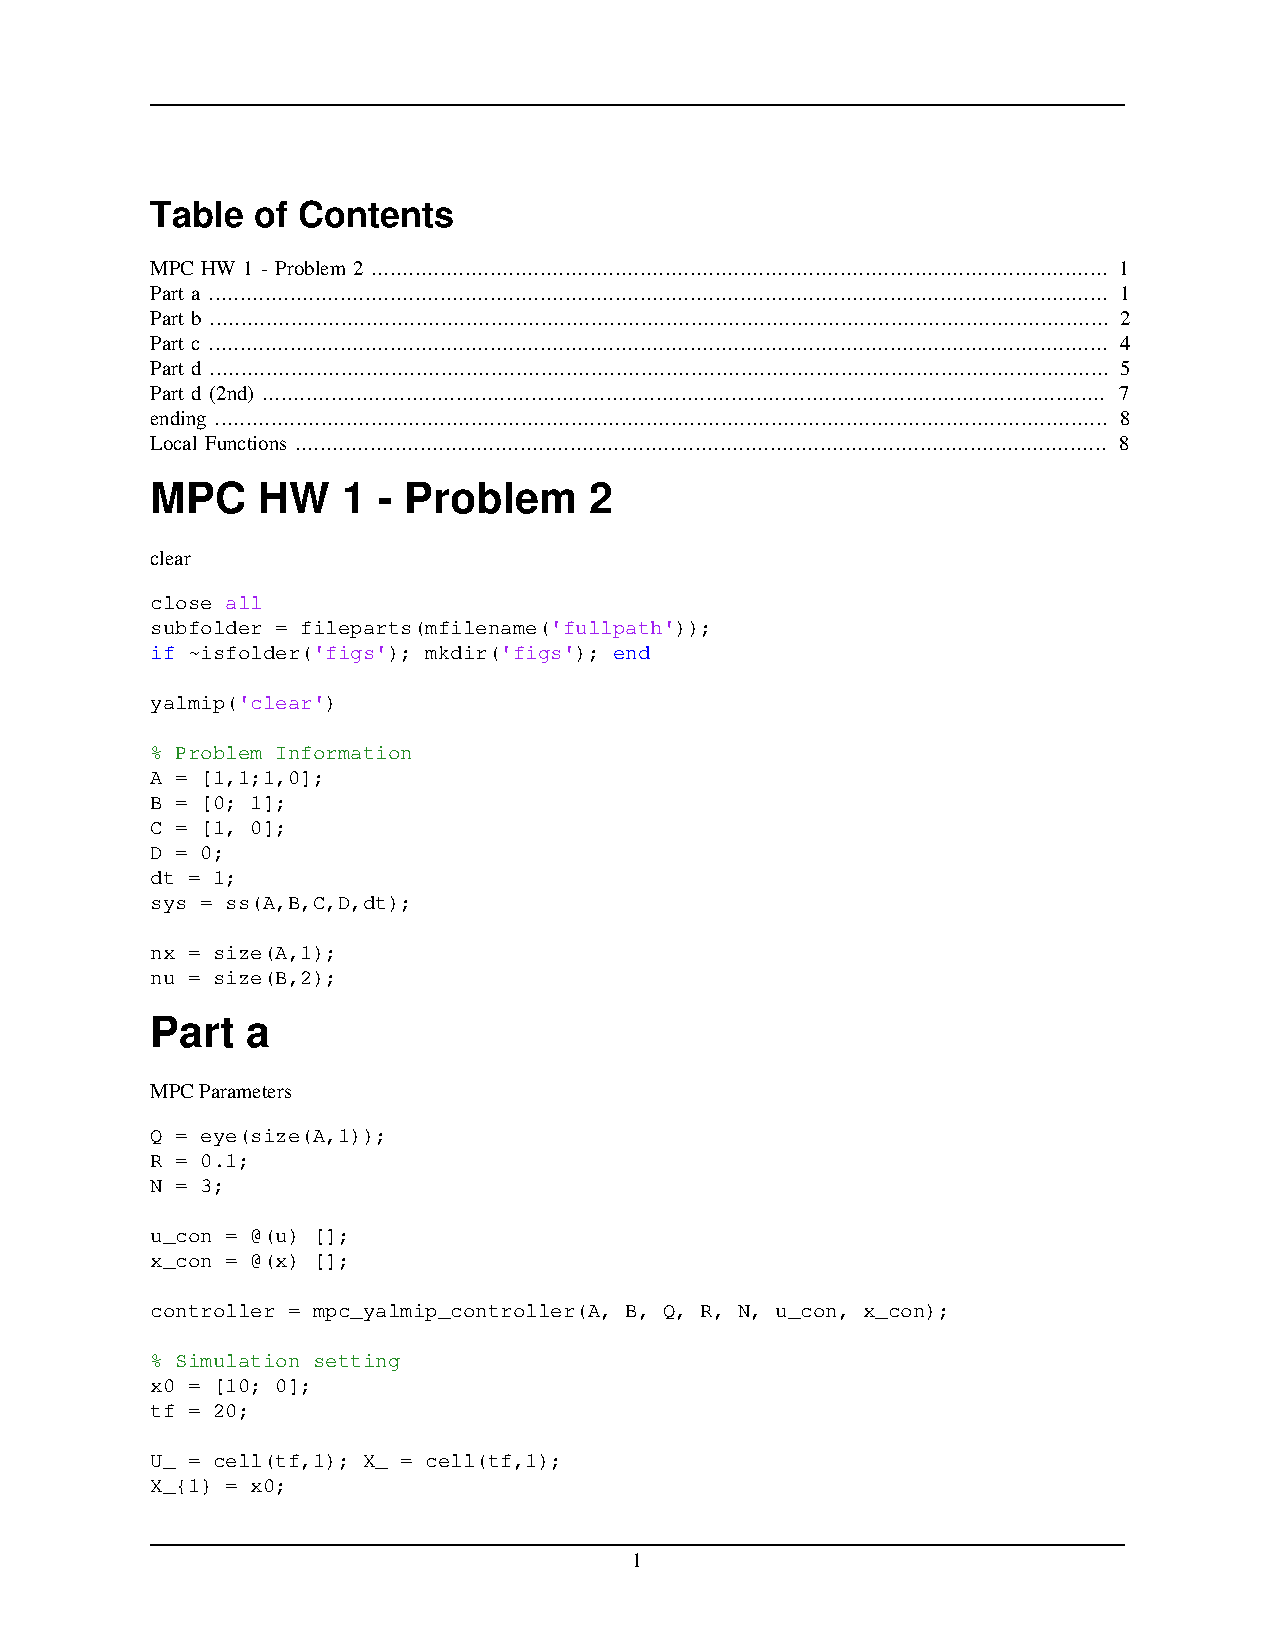
\includepdf[pages=-]{HW1_pblm2.pdf}


\end{document}



% \textbf{Dynamic Programming Implementation for Markov Decision Process}
% % Problem 1 ----------------------------------------------
% \section{Robot navigation in an uncertain environment} 
% \Problem
% You are designing a controller to navigate a robot through a cluttered and uncertain environment. 
% We use a very simplified 2D grid model, where the robot starts in the bottom-left corner, and must move to the top-right corner, and can move either up or to the right at each step.
% Due to unpredictable robot-environment interaction, if the robot moves in the same direction as in the previous time-step, there is a higher probability of moving in the desired direction than if it tries to change direction. 
% If the direction selected is the same as in the previous step, the robot lands in the desired state with probability 0.8 and lands in the undesired state with probability 0.2. 
% If the direction selected is different from in the previous step, the robot lands in the intended state with probability 0.6 and lands in the unintended state with probability 0.4. 
% The first move is treated as though there was a move in the same direction previously.

% The environment is a 41 $\cross$ 41 grid. Assume that at each time step, the robot knows its location in the grid and can use the information for feedback. 
% The environment has a number of obstacles whose locations are defined in the file \emph{robot\_nav.mat} available on eLearning. 
% Hitting an obstacle or the environment boundary results in a crash, and the mission is failed (i.e, you can treat the obstacle locations as absorbing states).

% \Solution
% A summary of the problem is as follows:

% Let the state be the robot position: \[
%     x_k \in \mathcal{X} = \{1,\dots,41\}^2 \subset \Z^2
% \]
% Obstacles exist within that result in a crash (along with the boundary), $\mathcal{X}_{obstacles}$, thus a safe region can be denoted as $\mathcal{X}_{safe} = \mathcal{X} \backslash \mathcal{X}_{obstacles}$.
% The initial state is in the SW corner: $x_{0} = \smqty[1\\1]$.
% Additionally, the goal state is in the NE corner: $x_{goal} = \smqty[41\\41]$.

% Let the input be the desired heading:\[
%     u_k \in \mathcal{U} = \qty{\text{N}, \text{E}} = \qty{\mqty[0\\+1], \mqty[+1\\0]}
% \]

% The update equation for the position is as follows:\[
%     x_{k+1} = f(x_k,u_k) = x_k + w_k(u_{k-1}) u_{k}, 
%     \quad w_k(u_{k},u_{k-1}) \sim \begin{cases}
%         \mqty[0.8 & 0.2 \\ 0.2 & 0.8] & u_{k} = u_{k-1}\\
%         \mqty[0.6 & 0.4 \\ 0.4 & 0.6] & u_{k} \neq u_{k-1}
%     \end{cases}
% \]

% You can model this as either augmenting the system with a previous time-step input to perform this simulation. 
% Alternatively, the objective 

% % 1a
% \subsection{}
% \Problem
% Determine and plot the optimal policy and value function for the stage cost $\forall_{k = 1,\dots, N}$ \[
%     g_k(x) = \begin{cases}
%         1 & x = x_{goal}\\%\text{goal state (NE-corner)}\\
%         -1 & x \in \mathcal{X}_{obstacles}\\%\text{obstacle location}\\
%         0 & \text{otherwise}
%     \end{cases}
% \]
% Comment on your result.
% \Solution

% See MATLAB code.

% The value function and optimal policy plots are shown in \autoref{fig:pblm1_valFunc} and \autoref{fig:pblm1_optPolicy} respectively.

% \begin{figure}[h]
%     \centering
%     % \includegraphics[width=0.5\textwidth]{figs/pblm1_valFunc.png}
%     \caption{Value function for problem 1.}
%     \label{fig:pblm1_valFunc}
% \end{figure}

% \begin{figure}[h]
%     \centering
%     % \includegraphics[width=0.5\textwidth]{figs/pblm1_optPolicy.png}
%     \caption{Optimal policy for problem 1. (yellow is East and blue is North)}
%     \label{fig:pblm1_optPolicy}
% \end{figure}

% The result is pretty much to be expected and makes sense logically.


% % 1b
% \subsection{}
% Simulate the system to estimate (via either distribution propagation or Monte Carlo) the success rate and plot a sample trajectory of a successful mission.


% The result for the controller seems to be either really terrible or the implimenation itself remains incorrect as the success rate is only around $13\%$.
% A sample of the successful trajectory is provided in \autoref{fig:pblm1_sampleTraj}.

% \begin{figure}[h]
%     \centering
%     % \includegraphics[width=0.5\textwidth]{figs/pblm1_sampleTraj.png}
%     \caption{Sample successful trajectory for problem 1.}
%     \label{fig:pblm1_sampleTraj}
% \end{figure}

% \newpage
% \textbf{Linear Quadratic Problems}
% % Problem 2 ----------------------------------------------
% \section{Non-zero Mean Disturbances}
% \Problem
% Use dynamic programming to derive the optimal const functions and policies for a linear quadratic problem with non-zero mean distrubances.
% The dynamcis are \[
%     x_{k+1} = A_k x_k + B_k u_k + w_k, \quad \forall_{k=0,\dots, N-1}
% \] 
% where $\mathbf{E} [w_k] = \bar{w}_k$ and $\mathbf{E}[w_k w_k^T] = W_k$, and the cost function is the linear quadradic cost: \[
%     \sum_{k=0}^{N-1} (x_k^T Q_k x_k + u_k^T R_k u_k) + x_N^T Q_N x_N
% \]

% Compute the optimal policy and optimal cost function for the problem instance with constant problem data $\forall_{k=0,\dots,N-1}$ \[
%     A_k = \mqty[
%         0.4 & -0.3 & 0 & 0.6\\
%         0.1 & -0.7 & 0.2 & 0\\
%         0.5 & 0.2 &-0.8 & 0.1\\
%         0 & 0.3 & -0.4 & 0.9
%     ], \quad 
%     B_k = \mqty[
%         0.1 & 0.1\\
%         0.1 & 0.3\\
%         0 & 0.1\\
%         0.2 & 0
%     ],
% \]
% $Q_k = \vb{I}$, $R_k = \vb{I}$, $\mathbf{E} [w_k] = \bar{w}_k = \smqty[0.1&-0.1&0.3&-0.3]^T$, $\mathbf{E}[w_k w_k^T] = W_k = 0.1 \vb{I}$, and $N = 30$.

% Report the optimal policy coefficients at time 0, $k=0$, and the optimal cost if the initial state is zero, $x_0 = \vb{0}$.

% \Solution
% The general dynamic programing algorithm for the time horizon, $N$, the terminal cost is set as $J_N(x_N) = g_{N}(x_N)$ and then minimizing the cost function for each time step recursively and then determines the optimal input and continues in reverse until $k=0$ to find the optimal policy $\pi_{k}^{\star}(x_k)$ $\forall_{k=0,\dots,N-1}$:\[
%     J_k(x_k) = \min_{u_k \in \mathcal{U}_k(x_k)} \vb{E}_w[
%         g_k(x_k,u_k,w_k) + J_{k+1}(f_k(x_k,u_k,w_k))
%         ]
% \] with $\pi_{k}^{\star}(x_k) = \arg \min$ of above.

% For the LQ case, the dynamic program can be defined by the algorithm with stage cost, $g_{k}(x_k,u_k) = x_k^T Q_k x_k + u_k^T R_k u_k$, and terminal cost, $g_{N}(x_N) = x_N^T Q_N x_N$.
% Initializing the terminal cost results in \[
%     J_N(x_N) = x_N^T Q_N x_N
% \] and then the recursive optimization for the LTV system becomes \[
%     J_k(x_k) =  \min_{u_k \in \mathcal{U}_k(x_k)} \vb{E}_w[
%         x_k^T Q_k x_k + u_k^T R_k u_k + J_{k+1}(A_k x_k + B_k u_k + w_k)
%     ]
% \]
% For simplicity, the quadratic form will be utilized and will be reduced to the LQ form, $x_k^T P_k x_k + r_k$, thus \[
%     J_N(x_k) = x_N^T Q_N x_N \implies P_N = Q_N, \ r_N = 0
% \] and the recursive iteration will also aim to reduce to an update for $P_k$ and $r_k$ as follows:
% \begin{align*}
%     J_k(x_k) &=  x_k^T P_k x_k + 2 q_k^T x_k + r_k \\
%     &= \min_{u_k \in \mathcal{U}_k(x_k)} \vb{E}_w[
%         x_k^T Q_k x_k + u_k^T R_k u_k + J_{k+1}(Ax_{k} + B u_{k} + w_k, u_{k+1}, w_{k+1})
%     ]
% \intertext{since $J_{k+1} = x_{k+1}^T P_{k+1} x_{k+1} + r_{k+1}$}
%     &= \min_{u_k \in \mathcal{U}_k(x_k)} \vb{E}_w[
%         x_k^T Q_k x_k + u_k^T R_k u_k 
%         + (A_k x_k + B_k u_k + w_k)^T P_{k+1} (A_k x_k + B_k u_k + w_k) 
%     \\ & \qquad \qquad \qquad 
%     + 2 q_{k+1}^T (A_k x_k + B_k u_k + w_k)
%         + r_{k+1}
%     ]
%     \\ %%%%%%%%%%%%%%%%%%%%%%%%%%%%%%%%%%%%%%%%%%%%%%
%     &= \min_{u_k \in \mathcal{U}_k(x_k)} \vb{E}_w[
%         x_k^T Q_k x_k 
%         + u_k^T R_k u_k 
%         + (x_k^T A_k^T + u_k^T B_k^T + w_k^T) P_{k+1} (A_k x_k + B_k u_k + w_k)
%     \\ & \qquad \qquad \qquad 
%     + 2 q_{k+1}^T (A_k x_k + B_k u_k + w_k)
%         + r_{k+1}
%     ]
%     \\ %%%%%%%%%%%%%%%%%%%%%%%%%%%%%%%%%%%%%%%%%%%%%%
%     &= \min_{u_k \in \mathcal{U}_k(x_k)} \vb{E}_w[
%         x_k^T Q_k x_k 
%         + u_k^T R_k u_k 
%         \\ & \qquad \qquad \qquad 
%         + \qty(
%             x_k^T A_k^T P_{k+1} A_k x_k
%             + x_k^T A_k^T P_{k+1} B_k u_k
%             + x_k^T A_k^T P_{k+1} w_k
%         )
%         \\ & \qquad \qquad \qquad 
%         + \qty(
%             u_k^T B_k^T P_{k+1} A_k x_k
%             + u_k^T B_k^T P_{k+1} B_k u_k
%             + u_k^T B_k^T P_{k+1} w_k
%         ) 
%         \\ & \qquad \qquad \qquad 
%         + \qty(
%             w_k^T P_{k+1} A_k x_k
%             + w_k^T P_{k+1} B_k u_k
%             + w_k^T P_{k+1} w_k
%         )
%         \\ & \qquad \qquad \qquad 
%         + \qty(
%             2 q_{k+1}^T A_k x_k
%             + 2 q_{k+1}^T B_k u_k
%             + 2 q_{k+1}^T w_k
%         )
%         + r_{k+1}
%     ]
% \intertext{Note that for scalar values the trace is equivalent and then the cyclic property of trace and linearity of expectation can be used to shift things around}
%     &= \min_{u_k \in \mathcal{U}_k(x_k)} \vb{E}_w[
%         x_k^T \qty(Q_k + A_k^T P_{k+1} A_k)
%         + u_k^T \qty(R_k + B_k^T P_{k+1} B_k) u_k
%         + x_k^T A_k^T P_{k+1} B_k u_k
%         + u_k^T B_k^T P_{k+1} A_k x_k
%     ]
%     \\ & \qquad \qquad \qquad 
%     + \vb{E}_w[
%         2 q_{k+1}^T A_k x_k
%         + 2 q_{k+1}^T B_k u_k
%         + r_{k+1}
%     ]
%     \\ & \qquad \qquad \qquad 
%     + \vb{E}_w[
%         x_k^T A_k^T P_{k+1} w_k
%         + w_k^T P_{k+1} A_k x_k
%     ]
%     \\ & \qquad \qquad \qquad 
%     + \vb{E}_w[
%         u_k^T B_k^T P_{k+1} w_k
%         + w_k^T P_{k+1} B_k u_k
%     ]
%     \\ & \qquad \qquad \qquad 
%     + \vb{E}_{w}[
%         w_k^T P_{k+1} w_k
%         + 2 q_{k+1}^T w_k
%     ]
%     \\ %%%%%%%%%%%%%%%%%%%%%%%%%%%%%%%%%%%%%%%%%%%%%%
%     &= \min_{u_k \in \mathcal{U}_k(x_k)}
%         x_k^T \qty(Q_k + A_k^T P_{k+1} A_k)
%         + u_k^T \qty(R_k + B_k^T P_{k+1} B_k) u_k
%         + x_k^T A_k^T P_{k+1} B_k u_k
%         + u_k^T B_k^T P_{k+1} A_k x_k
%     \\ & \qquad \qquad \qquad
%         + 2 q_{k+1}^T A_k x_k
%         + 2 q_{k+1}^T B_k u_k
%         + r_{k+1}
%     \\ & \qquad \qquad \qquad 
%     + 2 \trace(P_{k+1} \vb{E}_w[x_k^T w_k])
%     % \\ & \qquad \qquad \qquad 
%     + 2 \trace(P_{k+1} B_k \vb{E}_2[w_k^T u_k])
%     % \\ & \qquad \qquad \qquad 
%     + \trace(P_{k+1} \vb{E}_w[w_k^T w_k])
%     + 2 q_{k+1}^T \vb{E}[w_k]
%     \\ %%%%%%%%%%%%%%%%%%%%%%%%%%%%%%%%%%%%%%%%%%%%%%
%     &= 
%     x_k^T \qty(Q_k + A_k^T P_{k+1} A_k)
%     + 2 q_{k+1}^T A_k x_k
%     + 2 \trace(P_{k+1} \vb{E}_w[x_k^T w_k])
%     + \trace(P_{k+1} W_k)
%     + 2 q_{k+1}^T \bar{w}
%     + r_{k+1}
%     \\ & \qquad \qquad \qquad 
%     + \min_{u_k \in \mathcal{U}_k(x_k)}
%         u_k^T \qty(R_k + B_k^T P_{k+1} B_k) u_k
%         + 2 x_k^T A_k^T P_{k+1} B_k u_k
%         + 2 \trace(P_{k+1} B_k \vb{E}_w[w_k^T u_k])
% \end{align*}
% To solve this minimization, a derivative is performed w.r.t. $u_k$:
% \begin{align*}
%     0 &= \dv{u} \qty(
%         u_k^T \qty(R_k + B_k^T P_{k+1} B_k) u_k
%         + 2 x_k^T A_k^T P_{k+1} B_k u_k
%         + 2 q_{k+1}^T B_k u_k
%         + 2 \trace(P_{k+1} B_k \vb{E}_2[w_k^T u_k])
%     )\\
%     &= 2 \qty(R_k + B_k^T P_{k+1} B_k) u_k
%     + 2 x_k^T A_k^T P_{k+1} B_k
%     + 2 q_{k+1}^T B_k
%     + 2 \trace(P_{k+1} B_k \vb{E}_w[w_k^T])\\
%     &= (R_k + B_k^T P_{k+1} B_k) u_k
%     + x_k^T A_k^T P_{k+1} B_k
%     + q_{k+1}^T B_k
%     + \trace(P_{k+1} B_k \bar{w}_k^T)\\
%     -(R_k + B_k^T P_{k+1} B_k) u_k
%     &= x_k^T A_k^T P_{k+1} B_k
%     + \trace(P_{k+1} B_k w_k^T)\\
%     u_k &= -(R_k + B_k^T P_{k+1} B_k)^{-1} \qty(
%         x_k^T A_k^T P_{k+1} B_k
%         + q_{k+1}^T B_k
%         + \trace(P_{k+1} B_k \bar{w}_k^T)
%     )\\
%     u_k &= -(R_k + B_k^T P_{k+1} B_k)^{-1} \qty(
%         B_k^T P_{k+1} A_k) x_k
%         - (R_k + B_k^T P_{k+1} B_k)^{-1} \qty(q_{k+1}^T B_k + \trace(P_{k+1} B_k \bar{w}_k^T))
% \end{align*}
% Resulting an an optimal control law:\[
%     u_k^\star = K_k x_k + l_k
% \] with \[
%     K_k = -(R_k + B_k^T P_{k+1} B_k)^{-1} \qty(B_k^T P_{k+1} A_k)
% \] and \[
%     l_k = -(R_k + B_k^T P_{k+1} B_k)^{-1} \qty(q_{k+1}^T B_k + \trace(P_{k+1} B_k \bar{w}_k^T))
% \]

% Next, the cost function results is calculated recursively by
% \begin{align*}
%     J_{k}^{\star} &= x_k^T Q_k x_k + 2 q_k^T + r_k\\
%     &= x_k^T \qty(Q_k + A_k^T P_{k+1} A_k)
%     + 2 q_{k+1}^T A_k x_k
%     \\ & \qquad
%     + 2 \trace(P_{k+1} \vb{E}_w[x_k^T w_k])
%     + \trace(P_{k+1} W_k)
%     + 2 q_{k+1}^T \bar{w}
%     + r_{k+1}
%     \\ & \qquad 
%     + (-(R_k + B_k^T P_{k+1} B_k)^{-1} \qty(
%         x_k^T A_k^T P_{k+1} B_k
%         + q_{k+1}^T B_k
%         + \trace(P_{k+1} B_k \bar{w}_k^T)
%     ))^T \cdot
%     \\ & \qquad \qquad
%     \cdot \qty(R_k + B_k^T P_{k+1} B_k) (-(R_k + B_k^T P_{k+1} B_k)^{-1} \qty(
%         x_k^T A_k^T P_{k+1} B_k
%         + q_{k+1}^T B_k
%         + \trace(P_{k+1} B_k \bar{w}_k^T)
%     ))
%     \\ & \qquad 
%     + 2 x_k^T A_k^T P_{k+1} B_k (-(R_k + B_k^T P_{k+1} B_k)^{-1} \qty(
%         x_k^T A_k^T P_{k+1} B_k
%         + q_{k+1}^T B_k
%         + \trace(P_{k+1} B_k \bar{w}_k^T)
%     ))
%     \\ & \qquad 
%     + 2 \trace(P_{k+1} B_k \vb{E}_w[w_k^T (-(R_k + B_k^T P_{k+1} B_k)^{-1} \qty(x_k^T A_k^T P_{k+1} B_k
%         + q_{k+1}^T B_k
%         + \trace(P_{k+1} B_k \bar{w}_k^T)
%     ))])
% \end{align*}
% which when evaluated results in (after making an assumption of zero correlation between $x_k$ and $w_k$) \[
%     \begin{split}
%         J_{k+1}(x)
%         &=  x^T[(Q+A^TP_{k+1}A)-(A^TP_{k+1}^TB^T)(R+B^TP_{k+1}B)^{-1}]x\\
%         &+  2\bar{w}^T[(P_{k+1}A)-(R+B^TP_{k+1}B)^{-1}(BP_{k+1}A)]x\\
%         &+ \bar{w}^T[(P_{k+1}^TB)(R+B^TP_{k+1}B)-(B^TP_{k+1})]\bar{w}\\
%         &+ \mathbf{tr}(P_{k+1}W_t) + r_{k+1}
%     \end{split}    
% \]
% where 
% \(P = (Q+A^TP_{k+1}A)-(A^TP_{k+1}^TB^T)(R+B^TP_{k+1}B)^{-1}\), 
% \(Q = (P_{k+1}A)-(R+B^TP_{k+1}B)^{-1}(BP_{k+1}A)\), 
% and \(R = (P_{k+1}^TB)(R+B^TP_{k+1}B)-(B^TP_{k+1}) + \mathbf{tr}(P_{k+1}W_t) + r_{k+1}\).



% As for a final result, results (calculated in matlab) for the total cost at $k=0$, with $N = 30$ is $J_0 = 6.0635\cross 10^3$.








% % % Appendix ----------------------------------------------
% % \newpage
% \appendix
% % \bibliographystyle{plain}
% % \bibliography{refs.bib}

% \newpage
% % \includepdf[pages=-]{MECH6326_HW4.pdf}


